\begin{frame}
\newcommand{\song}{\setCJKfamilyfont{song}}
\newcommand{\xiaoer}{\fontsize{18pt}{18pt}\selectfont}
	\begin{center}
	{\song\xiaoer\textbf{人工蜂群算法}}
	\end{center}
\end{frame}

\begin{frame}
  \frametitle{ABC算法背景}
	\qquad 人工蜂群算法(Attificial Bee Colony,ABC)是由土耳其学者Karaboga于2005年提出,其基本思想是启发 	 	于蜂	群通过个体分工和信息交流,相互协作完成采蜜任务。与传统的优化方法相比,它的主要优点是不需要了解问    	题的特殊信息,只需要对问题进行优劣比较,通过人工蜂群个体的局部寻优行为,最终在群体中使得全局最优值	 	凸现出来,具有较快的收敛速度。但同时也存在以下问题:ABC算法存在“早熟”的收敛性缺陷,即在接近全局最优解时,已陷入局部最优。

\end{frame}

\begin{frame}
	\frametitle{自然界的蜂群}
	\begin{columns}
	\column{.4\textwidth}
		\begin{itemize}
			\item { 3个基本要素}
				\begin{itemize}
					\item { 蜜源Food Source}
					\item { 被雇佣蜂(引领峰)Employed Foragers}
					\item { 未被雇佣蜂Unemployed Foragers}
						\begin{itemize}
							\item { 跟随蜂 }
							\item { 侦查蜂 }
						\end{itemize}
				\end{itemize}
			\item { 2种基本行为}
				\begin{itemize}
					\item {为蜜源招募蜜蜂Recruit}
					\item {放弃蜜源Abandon}
				\end{itemize}
			 \item { 信息交流}
				\begin{itemize}
					\item {舞蹈区:摇摆舞}
				\end{itemize}
		\end{itemize}
	\column{.6\textwidth}
		\begin{itemize}
			\item[ ] 
				\begin{figure}[htbp]
					\centering
					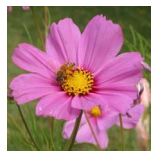
\includegraphics[scale=0.5]{pic/bee1.png}
				\end{figure}
			\item[ ]
				\begin{figure}[htbp]
					\centering
					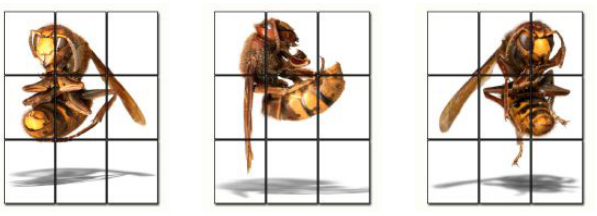
\includegraphics[scale=0.5]{pic/bee2.png}
				\end{figure}
			\item[ ] 
				\begin{figure}[htbp]
					\centering
					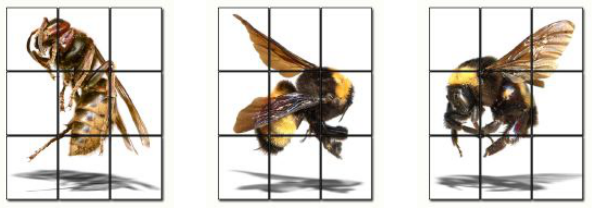
\includegraphics[scale=0.5]{pic/bee3.png}
				\end{figure}
		\end{itemize}
	\end{columns}
\end{frame}


\begin{frame}
	\frametitle{自然界的蜂群}
	\begin{columns}
	\column{.6\textwidth}
		\begin{itemize}
			\item {引领蜂的搜索行为}
				\begin{itemize}
					\item {在舞蹈区进行蜜源信息分享后,发现自己的蜜源质量并不高,放弃蜜源重新变成侦查蜂寻找新蜜源(图中UF线)}
					\item {在舞蹈区跳摇摆舞招募蜜蜂,此时蜂巢里的非雇佣蜂以一定概率跟随引领蜂回到蜜源进行采蜜(图中EF1线)}
					\item {继续在蜜源处采蜜而不进行招募(图中EF2)}
				\end{itemize}
			\item {非雇佣蜂的搜索行为}
				\begin{itemize}
					\item {以侦查蜂的身份,自发搜索蜂巢附近的蜜源(图中S线)}
					\item {在观察完摇摆舞被雇佣成为跟随蜂,开始搜索对应蜜源附近并采蜜(图中R线)}
				\end{itemize}
		\end{itemize}
	\column{.4\textwidth}
		\begin{figure}[htbp]
			\centering
			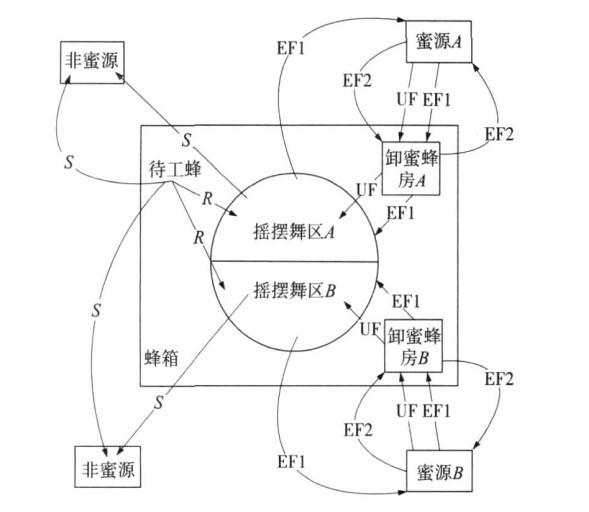
\includegraphics[width=6cm]{pic/bee4.jpg}
		\end{figure}
	\end{columns}
\end{frame}


\begin{frame}
	\frametitle{自然界的蜂群}
	\begin{columns}
	\column{.6\textwidth}
		\begin{itemize}
			\item {角色转换}
				\begin{itemize}
					\item {引领蜂用于维持优良解(记录当前局部最优解)。}
					\item {跟随蜂用于提高收敛速度(搜索局部最优解的附近空间)。}
					\item {侦查蜂用于增强摆脱局部最优的能力(重新全局搜索)。}
				\end{itemize}
		\end{itemize}
	\column{.4\textwidth}
		\begin{figure}[htbp]
			\centering
			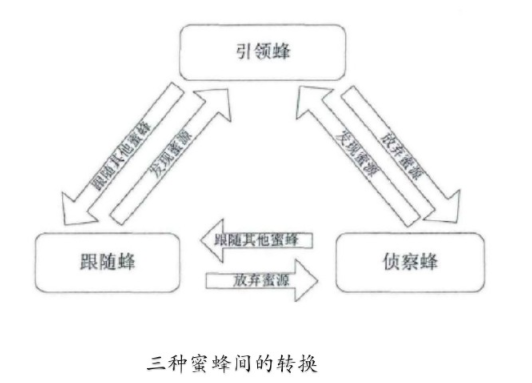
\includegraphics[width=6cm]{pic/bee5.png}
		\end{figure}
	\end{columns}
\end{frame}

\begin{frame}
	\frametitle{ABC算法模型}
	\begin{columns}
	\column{.6\textwidth}
	\qquad 首先初始化种群,派出侦查蜂搜索蜜源,找到蜜源后转换为引领蜂并评估蜜源的质量,所有引领蜂搜索完毕后回到蜂巢,令适应度高的蜜源对应的引领蜂招募跟随蜂,并对蜜源进行邻域搜索,保留较好的解;令适应度低的蜜源对应的引领蜂重新成为侦查蜂搜索新的蜜源,不断循环输出最优解。
	\column{.4\textwidth}
	\begin{table}[]
	\centering
	\caption{采蜜行为与优化问题的映射}
	\label{采蜜行为与优化问题的映射}
	\begin{tabular}{ccll}
	\cline{1-2}
	\multicolumn{1}{|c|}{\textbf{蜂群采蜜行为}} & \multicolumn{1}{c|}{\textbf{优化问题}} &  &  \\ \cline{1-2}
	\multicolumn{1}{|c|}{蜜源位置}            & \multicolumn{1}{c|}{可行解}            &  &  \\ \cline{1-2}
	\multicolumn{1}{|c|}{蜜源质量}            & \multicolumn{1}{c|}{适应度}            &  &  \\ \cline{1-2}
	\multicolumn{1}{|c|}{采蜜速度}            & \multicolumn{1}{c|}{收敛速度}           &  &  \\ \cline{1-2}
	\multicolumn{1}{|c|}{食物源质量最大值}        & \multicolumn{1}{c|}{最优解}            &  &  \\ \cline{1-2}
	\multicolumn{1}{l}{}                  & \multicolumn{1}{l}{}                &  & 
	\end{tabular}
	\end{table}
	\end{columns}
\end{frame}



\begin{frame}
	\frametitle{1. 蜜源初始化}
	\begin{itemize}
		\item { 设解空间的维度为D,初始蜜源的个数为NP,控制参数limit(局部搜索次数阈值)和最大循环数MaxCycle等。}
		\item { 将蜂群分为引领蜂、侦查蜂、跟随蜂三个类型,且引领蜂和跟随蜂各占蜂群的一半,且其数量等于NP。}
		\item { 根据(1)(2)式在搜索空间随机产生NP个蜜源,并为每一个蜜源分配一个引领蜂。 }
			\begin{equation}
				\vec{X}_{i} = [x_{i1}, x_{i2}, ... x_{iD}]   
			\end{equation}
			\begin{equation}
				x_{id} = L_{d} + rand(0,1) * (U_{d} - L_{d}) 
			\end{equation}
			其中$U_{d}$,$L_{d}$分别表示搜索空间的上限和下限。
	\end{itemize}
\end{frame}

\begin{frame}
	\frametitle{2.搜索更新}
	\begin{itemize}
		\item { 在搜索的开始阶段,引领蜂首先计算蜜源的适应度,如(3)式所示。}
			\begin{equation}
				fit_{i} = \left\{  
             		\begin{array}{lr}  
             		1 / (1 + f_{i}),f_{i} \geq 0 &  \\  
             		1 + abs(f_{i}), otherwise    
             	\end{array}  
           		\right.    
			\end{equation}
			其中$f_{i}$表示解的函数值。
		\item { 再在蜜源i的附近根据(4)式搜索一个新的蜜源 $ V_{i} = [v_{i1},v_{i2},... v_{iD}] $,当新蜜源的适应度fit优于xi时,采用贪婪选择方法用新蜜源替代原来的蜜源,否则保留。}
		\item { 当所有的引领蜂完成贪婪选择后,回到蜂巢舞蹈区进行交流蜜源信息。} 
	\end{itemize}
	\begin{equation}
		v_{id} = x_{id} + \varphi * (x_{id} - x_{jd})    
	\end{equation}
	\qquad 其中$ j \neq i $, 表示在NP个蜜源中随机选择一个不等于i的蜜源;$ \varphi $是[-1,1]均匀分布的随机数。
\end{frame}

\begin{frame}
	\frametitle{3.招募跟随蜂}
	\begin{itemize}
		\item {跟随蜂根据引领蜂分享的蜜源信息,按式(5)的方式计算概率并选择跟随,并采用如2一样的贪婪选择方法在所对应的蜜源附近搜索局部最优解。}
	\end{itemize}
	\begin{equation}
	p_{i} = fit_{i} / \sum_{i=1}^{NP} fit_{i}
	\end{equation}
\end{frame}

\begin{frame}
	\frametitle{4.产生侦查蜂}
	\begin{itemize}
		\item {在搜索过程中,若对蜜源Xi邻域的搜索次数达到limit而未找到更好的蜜源,则该蜜源会被放弃,与之对应的引领蜂会变成侦查蜂,如(6)式所示重新在全局空间随机搜索一个新的蜜源。}
	\end{itemize}
	\begin{equation}
	X_{i}^{t+1} = \left\{  
             		\begin{array}{lr}  
             			L_{d} + rand(0,1) * (U_{d} - L_{d}),t_{i} \geq limit &  \\  
             			X_{i}^{t}, otherwise    
             		\end{array}  
              \right.
	\end{equation}
	\begin{itemize}
		\item {记录当前所有蜜蜂找到的最优蜜源,并跳至第2步,重新迭代直到满足最大迭代次数MaxCycle或者小于优化误差时,输出全局最优解。}
	\end{itemize}
\end{frame}

\begin{frame}
	\frametitle{ABC算法框架}
	\begin{algorithm}[H]
	\caption{ABC}\label{bee_alg}
	\algsetup{linenosize=\tiny} \scriptsize
		\begin{algorithmic}
			\STATE{Initialize the food sources $X_i(i=1,2,3,...,n)$ by Eq.1,\\ 
			the colony count,NP; control parameter,limit; the Max cycle count, MaxCycle;}
			
			\FOR {cycle from 1 to MaxCycle do}
				\FOR {each employee bee i do}
					\STATE {Choose a food source $X_{k}$ in the neighbourhood of $X_{i}$; }
					\STATE {select a jth dimension above all dimension;}
					\STATE {Genernate a food source vi in the neighborhood of $x_{i}$ and $x_{k}$ by Eq.2;}
					\STATE {Apply greedy selection between of $x_{i}$ and $x_{k}$;}
				\ENDFOR
				\FOR {each onlooker bee i do}
					\STATE {select a food source $X_{i}$ depending on probability pi using Eg.3; }
					\STATE {Choose a food source $X_{k}$ in the neighbourhood of $X_{i}$; }
					\STATE {Genernate a food source vi in the neighborhood of $x_{i}$ and $x_{k}$ by Eg.2;}
					\STATE {Apply greedy selection between of $x_{i}$ and $x_{k}$;}
				\ENDFOR
				\IF {there exits an abondoned food source}
					\STATE {Scout bee determines a new food source by Eq.1; }
				\ENDIF
				\STATE {Update best food source;}
			\ENDFOR
		\end{algorithmic}
	\end{algorithm}
\end{frame}

\begin{frame}
	\frametitle{比较}
	\begin{table}[!htbp]
		\centering
		\caption{Numerical benchmark function}
		\label{my-label}
		\begin{tabular}{|c|c|c|cc}
		\cline{1-2}
		Name     		& function  														& range 		&  &  \\ \cline{1-3}
		Sphere函数 		& $f_{1}(x)= \sum_{i=1}^d x_{i}^2 $     							& [-100,100]	&  &\\ \cline{1-3}
		Rosenbrock函数	& $f_{2}(x)= \sum_{i=1}^d (100(x_{i+1}-x_{i}^2)^2 + (x_{i} - 1)^2 ) $ 	& [-30,30] 		&  &  \\ \cline{1-3}
		Griewank函数    	& $f_{3}(x)= \frac{1}{4000} \sum_{i=1}^d x_{i}^2 -  \prod_{i=1}^d cos(\frac{x_{i}}{\sqrt{i}}) + 1 $   	& [-600,600]	&  &  \\ \cline{1-3}
		Rastrigin函数   	& $f_{4}(x)=\sum_{i=1}^d (x_{i}^2 - 10cos(2   \pi 2 x_{i} + 10)$     	& [-5.12,5.12] 	&  &  \\ \cline{1-3}
		\end{tabular}
	\end{table}

	其中函数 $ f_{1}(x) $是单峰函数; 函数 $ f_{2}(x) $ 是很难极小化的病态函数; 函数 $ f_{3}(x) $, $ f_{4}(x) $都是具有大量局部最优点的多峰函数,

\end{frame}

\begin{frame}
	\frametitle{比较}

	\begin{figure}[htbp]
			\centering
			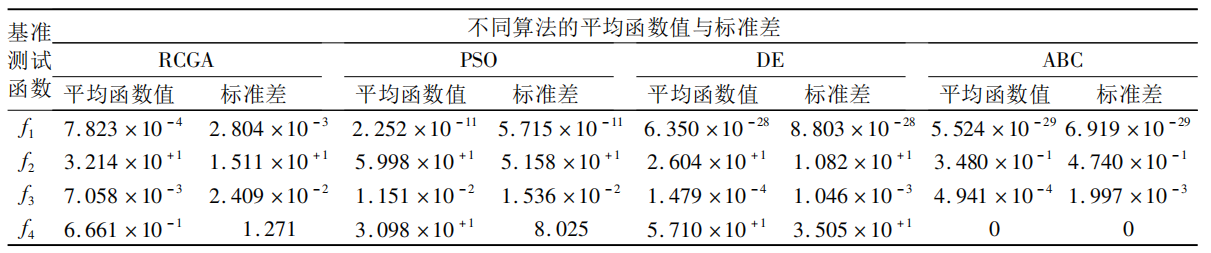
\includegraphics[width=1.0\textwidth]{pic/bee10.png}
			\caption{四种算法运行平均最优值比较}
			\label{fig:pt3}
	\end{figure}

\end{frame}

\begin{frame}
	\frametitle{比较}

		\begin{figure}[htbp]
			\centering
			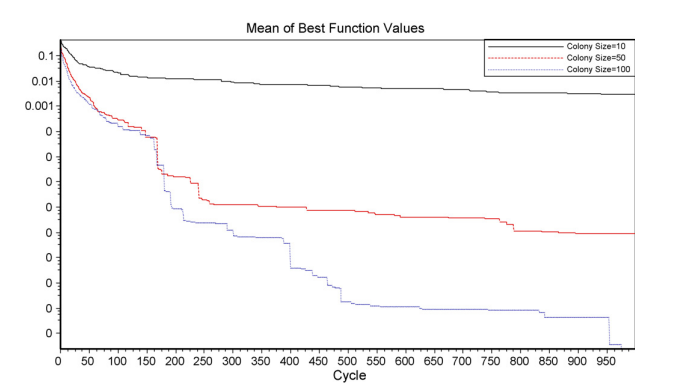
\includegraphics[width=0.4\textwidth]{pic/bee11.png}
			\caption{四种算法测试最小数随迭代次数的变化过程曲线}
			\label{fig:pt4}
		\end{figure}


\end{frame}

\begin{frame}
	\frametitle{改进}
	\begin{itemize}
		\item {基于混沌鲶鱼效应的人工蜂群算法:一方面通过使用混沌映射的方法替代原来的一般随机化初始蜜源过程;另一方面,将鲶鱼效应施加到蜜蜂种群内,并以混沌波动的方式衍生出一种新型的混沌鲶鱼蜂,用来替代原侦查蜂负责搜索新蜜源的任务,且同原蜂群个体之间形成了有效的竞争、协作机制}
		\item {搜索机制的改进:采用局部随机搜索算子对当前最优蜜源进行局部搜索,以加快搜索速度,同时利用基于排序的选择概率替代原算法中直接利用适应度计算的概率,来保证解的多样性。}
	\end{itemize}
\end{frame}


\begin{frame}
	\frametitle{Application:TSP问题}
	\begin{columns}
	\column{.6\textwidth}
	\qquad 给定N个城市 $C=(C_{1},C_{2}...C_{N})$,求一条从一个城市出发拜访N个所有城市的道路 $(C_{n1},C_{n2}...C_{nN})$,且每个城市有且仅能访问一次,最终回到开始的城市,其中任意两个城市的距离为d(Ci,Cj),使得求得的路径距离最小。
	\column{.4\textwidth}
	\begin{figure}[htbp]
		\flushleft
		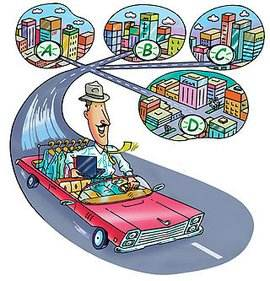
\includegraphics[width=3cm]{pic/bee6.jpg}
		\caption{TSP问题}
	\end{figure}
	\end{columns}
\end{frame}


\begin{frame}
	\frametitle{TSP问题}
	\begin{columns}
	\column{.6\textwidth}
	\qquad 所有城市的任一种排列即是问题的一个解,因此初始解空间就是N个城市的排列组合。在人工蜂群算法中,将城市个数N作为解空间的维度,每一个蜜源的位置表示其中一个路径的组合,用这条路径的距离长度表示蜜源的适应度,也就是说,适应度越小的蜜源,所表示的路径也就最优。\\
	\qquad 引领蜂和跟随蜂在更新蜜源位置时,是选择其对应的路径中任意两处进行调换生成新的路径,表示新的位置。
	\column{.4\textwidth}
	\begin{table}[]
	\centering
	\caption{TSP与ABC算法映射}
	\label{my-label}
	\begin{tabular}{|l|l|lll}
	\cline{1-2}
	TSP问题     & ABC算法  &  &  &  \\ \cline{1-2}
	访问所有城市的路径 & 蜜源位置   &  &  &  \\ \cline{1-2}
	路径长度      & 蜜源的适应度 &  &  &  \\ \cline{1-2}	
	最短路径      & 最优蜜源   &  &  &  \\ \cline{1-2}
	\end{tabular}
	\end{table}
	\end{columns}
\end{frame}

\begin{frame}
	\frametitle{算法框架}
	\begin{algorithm}[H]
	\caption{ABC on  TSP}\label{bee_alg}
	\algsetup{linenosize=\tiny} \scriptsize
		\begin{algorithmic}
			\STATE{Initialize the parameter: colony size N, maximum number of iteration MaxCycle, limit.}
			\STATE{Initialize the food sources $x_i(i=1,2,3,...,N)$ and compute the fit value.}
			
			\FOR {cycle from 1 to MaxCycle do}
				\FOR {each employee bee i do}
					\STATE {produce a food source $v_{i}$ in the neighbourhood of $X_{i}$; }
					\STATE {Apply greedy selection between of $x_{i}$ and $v_{i}$;}
				\ENDFOR
				\FOR {each onlooker bee i do}
					\STATE {select a food source $x_{i}$ depending on probability pi ; }
					\STATE {produce a food source $v_{i}$ in the neighbourhood of $X_{i}$; }
					\STATE {Apply greedy selection between of $x_{i}$ and $v_{i}$;}
				\ENDFOR
				\IF {there exits an abondoned food source}
					\STATE {Scout bee determines a new food source. }
				\ENDIF
				\STATE {Update best food source;}
			\ENDFOR
		\end{algorithmic}
	\end{algorithm}
\end{frame}

\begin{frame}
	\frametitle{仿真实验}
	\begin{figure}[htbp]
	\begin{minipage}[t]{4cm}
	\centering  
	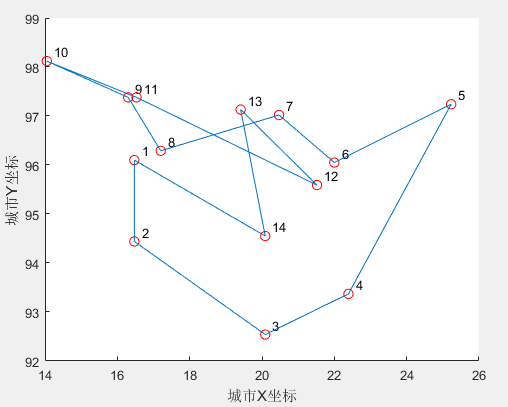
\includegraphics[width=4cm]{pic/bee7.png}  
	\caption{初始路径图}
	\end{minipage}  
	\begin{minipage}[t]{4cm}
	\centering  
	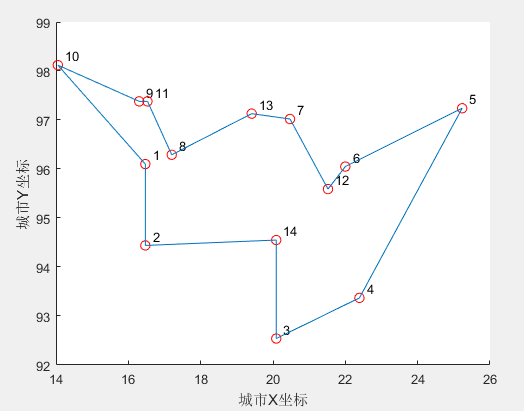
\includegraphics[width=4cm]{pic/bee8.png}  
	\caption{结果路径图}
	\end{minipage}  
	\begin{minipage}[t]{4cm}  
	\flushright
	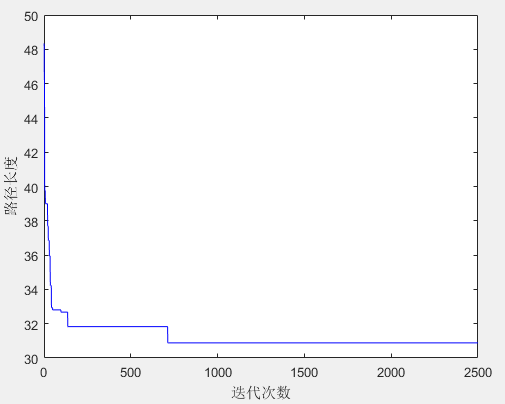
\includegraphics[width=4cm]{pic/bee9.png}  
	\caption{优化曲线}  
	\end{minipage}  
	\end{figure}  
\end{frame}


\begin{frame}
	\frametitle{参考文献}
	\begin{thebibliography}{123456} 
	\bibitem{bee_bib1} 何尧,刘建华,杨荣华.人工蜂群算法研究综述[J/OL].计算机应用研究,2018(05):1-8
	\bibitem{bee_bib2} 陈阿慧,李艳娟,郭继峰.人工蜂群算法综述[J].智能计算机与应用,2014,4(06):20-24
	\bibitem{bee_bib3} Karaboga D. An idea based on honey bee swarm for numerical optimization[R]. Technical report-tr06, Erciyes university, engineering faculty, computer engineering department, 2005.
	\bibitem{bee_bib4} 王慧.人工蜂群算法的性能比较研究[J].河北工程技术高等专科学校学报,2015(01):41-44.
	\bibitem{bee_bib5} 王生生,杨娟娟,柴胜.基于混沌鲶鱼效应的人工蜂群算法及应用[J].电子学报,2014,42(09):1731-1737.
	\bibitem{bee_bib6} 黄秋菀, 王志刚, 夏慧明. 求解旅行商问题的人工蜂群算法 [J]. 价值工程,2013,32(09):206-207
	
	\end{thebibliography}
\end{frame}
